 \section{Introdução}

  \begin{frame}{Motivação}
     \begin{itemize}
      \item Este trabalho é uma contribuição para \emph{software} livre em sistemas distribuídos.
      \item Armazenamento de dados $===>$ componente essencial na computação de alto desempenho. 
      \item Códigos Corretores de Erro (\emph{Erasure codes}) introduzem redundância para alcançar confiabilidade e redução do custo de armazenamento.    
     \end{itemize}
  \end{frame}

  \begin{frame}{Motivação}
   \begin{figure}[h]
     \centering
     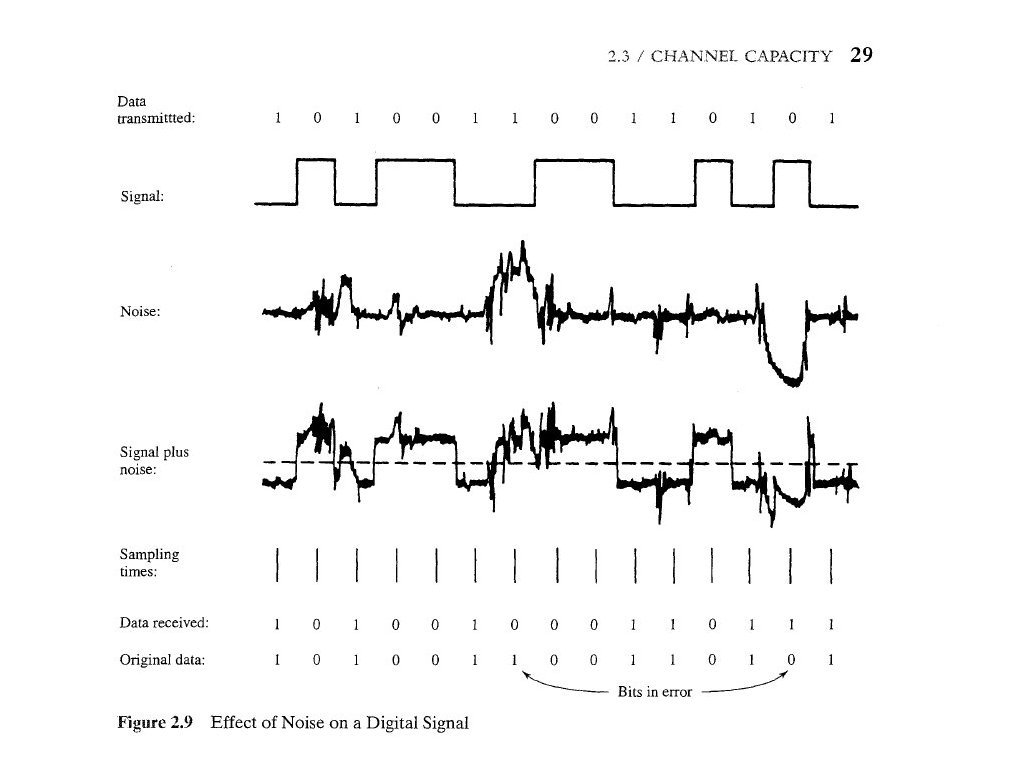
\includegraphics[scale=.25]{stalling-channel-capacity.jpg}
     \caption{Efeito do ruído no sinal digital \cite{Stallings:2005}}
     \label{fig1:ersd}
   \end{figure}
  \end{frame}

  \begin{frame}{Motivação}
     \begin{itemize}
         \item Popularização dos computadores e as pesquisas espaciais $==>$ os códigos corretores de erros tornaram-se parte comum de comunicações por satélite, de redes de computadores, de armazenamento em discos óticos e outros meios magnéticos.
         \item Uso frequente em nosso cotidiano
%quando se assiste a um programa de televisão, quando se ouve música a partir de um CD, quando se atende um telefonema, quando se assiste um filme gravado em DVD, quando se navega pela internet.
     \end{itemize}
  \end{frame}

% http://worldtelevisao.blogspot.com.br/2011/05/programas-infantis-que-fizeram-historia.html
  \begin{frame}{Motivação}
   \begin{figure}[h]
     \centering
     
\includegraphics[scale=.3]{enio-beto.jpg}
     \caption{Assistir programa de televisão Vila Sésamo\cite{WTPI:2012}}
     \label{fig7:tv}
   \end{figure}

% http://vidaanascer.blogspot.com.br/2012/09/notas-da-alma.html
   \begin{figure}[h]
     \centering
     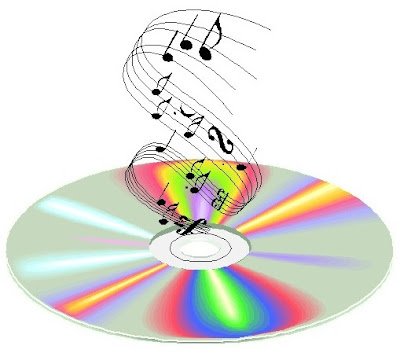
\includegraphics[scale=0.2]{music_cd.jpg}
     \caption{Ouvir música a partir de um CD\cite{MNA:2012}}
     \label{fig8:cd}
   \end{figure}
  \end{frame}

  \begin{frame}{Motivação}
% http://volneyf.blogspot.com.br/2008_04_01_archive.html
   \begin{figure}[h]
     \centering
     
\includegraphics[scale=0.3]{telephone-ringing.jpg}
     \caption{Atender um telefonema\cite{VF:2012}}
     \label{fig9:tel}
   \end{figure}


% http://phpbrasil.com/artigo/ozk4KmI6_tdC/2/criando-sites-para-celular-com-wml-parte-1
   \begin{figure}[h]
     \centering
     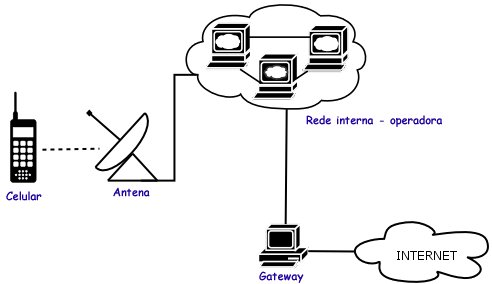
\includegraphics[scale=0.2]{internet-celular.jpg}
     \caption{Navegar pela internet\cite{FBP:2012}}
     \label{fig10:internet}
   \end{figure}
  \end{frame}

  \begin{frame}{Motivação}
     \begin{itemize}
      \item Alguns sistemas que utilizam códigos corretores de erros:
	\begin{itemize}
%           \item \emph{Digital Fountain} (\emph{multicasting} multimídia confiável)\cite{Byers:1998}
            \item \emph{NASA's Deep Space Network} no envio e na recepção de sinais e dados de telemetria
(\emph{downlinks}) vindos de veículos espaciais (\emph{very distant spacecrafts}) e para enviar telecomandos (\emph{uplinks}) para
% veículos espaciais \cite{Abrantes:2010, Almeida:2007, STO:2010, TDD:2010};
veículos espaciais;
%           \item \emph{Delay and Disruption Tolerant Networks}, redes de sensores e redes~\emph{peer-to-peer} \cite{Bhagwan:2004, Alencar:2004, Haeberlen:2005, Houri:2009,RTAD:2007, Rodrigues:2005, Wilcox-O'Hearn:2008};
           \item \emph{Delay and Disruption Tolerant Networks}, redes de sensores e redes~\emph{peer-to-peer};
%           \item armazenamento de grande volume de dados \cite{Anderson:1998,Kubiatowicz:2000,  Saito:2004, Schmuck:2002, Storer:2008,
% Storer:2009, Xia:2006}, como também o sistema de arquivos distribuído do Hadoop (HDFS)~\cite{HDFS-503:2010}.
           \item armazenamento de grande volume de dados, como também o sistema de arquivos distribuído do Hadoop (HDFS).
%           \item sistema de arquivos distribuído do Hadoop (HDFS)~\cite{HDFS-503:2010}
	\end{itemize}
     \end{itemize}
  \end{frame}

% http://www2.jpl.nasa.gov/basics/bsf10-1.php

%  \begin{frame}{Motivação}
%   \begin{figure}[h]
%     \centering
%     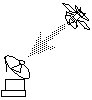
\includegraphics[scale=.3]{1-way.jpg}
%     \caption{1-\emph{way}: dados vindos de um veículo espacial\cite{Plank:2004}}
%     \label{fig2:1way}
%   \end{figure}
%   \begin{figure}[h]
%     \centering
%     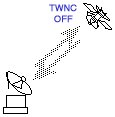
\includegraphics[scale=0.3]{2-way.jpg}
%     \caption{2-\emph{way}: dados vindos de um veículo espacial e comandos enviados para um veículo espacial\cite{Plank:2004}}
%     \label{fig3:2way}
%   \end{figure}
%   \begin{figure}[h]
%     \centering
%     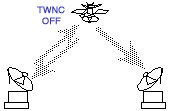
\includegraphics[scale=0.3]{3-way.jpg}
%     \caption{3-\emph{way}: dados vindos de dois veículos espaciais e comandos enviados para dois veículos espaciais\cite{Plank:2004}}
%     \label{fig4:3way}
%   \end{figure}
%  \end{frame}

% http://www.au.af.mil/au/awc/awcgate/jplbasic/bsf10-1.htm
% Two-Way Non-Coherent

  \begin{frame}{Motivação}
   \begin{figure}[h]
     \centering
     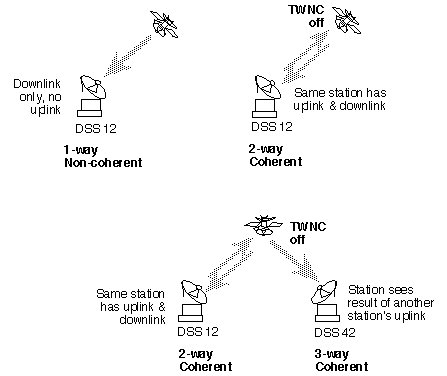
\includegraphics[scale=.4]{bsfii6.jpg}
     \caption{\emph{NASA's Deep Space Network}\cite{JPLCIT:2012}}
     \label{fig2:nasa}
   \end{figure}
  \end{frame}

% Venturebeat.com/2012/11/14/facebook-north-carolina-data-center/
  \begin{frame}{Motivação}
   \begin{figure}[h]
     \centering
     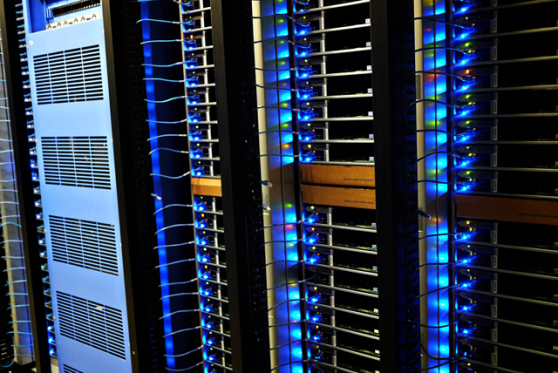
\includegraphics[scale=.5]{facebook-data-center.jpg}
     \caption{Dezenas de milhares de \emph{Open Computer Machines} do Facebook \emph{data center} em Forest City, North Carolina, USA
\cite{VBFB:2012}}
     \label{fig5:fdc}
   \end{figure}
  \end{frame}

  \begin{frame}{Motivação}
     \begin{itemize}
      \item O HDFS, por padrão, implementa alta disponibilidade dos dados via replicação simples dos blocos de dados. Esta abordagem acarreta um alto custo de armazenamento para garantir que os dados estarão sempre disponíveis.
      \item Esforços iniciais $===>$ \emph{Redundant Array of Independent Drives} (RAID)~\cite{HDFS-503:2010,Patterson:1988} e mais recentemente, Reed-Solomon (RS)~\cite{MR-1969:2010}.
     \end{itemize}
  \end{frame}


  \begin{frame}{Motivação}
     \begin{itemize}
        \item RAID (\emph{Redundant Arrays of Inexpensive [Independent] Disks} (RAID), do ponto de vista de suas estruturas algébricas, é uma classe de códigos de blocos lineares.
        \item RAID é um método para prover tolerância a falhas ou alto desempenho em sistemas de armazenagem utilizando, para isso, distribuição de dados em diferentes dispositivos e uma codificação de correção de erros ou paridade ou replicação de dados~\cite{Ramakrishnan:2003}.
        \item RAID foi introduzido por D. A. Patterson na Universidade da California, Berkeley (UC Berkeley) em 1988 \cite{Patterson:1988}.
        \item O código fonte do Hadoop implementa RAID-5, que na sua versão clássica, "fatia" dados e paridade, através dos discos, como num arranjo. A única paridade é calculada através da operação \emph{bitwise} XOR. 
     \end{itemize}
  \end{frame}

% \footnote{Essa definição foi apresentada pelo Prof.dr.ir Henk C.A. Van Tilborg, pesquisador da Technische Universiteit Eindhoven, na sua palestra Old and New(er) Results in the Theory of Burst-Correcting Codes em 23 de novembro no Instituto de Matemática, Estatística e Computação Científica da Universidade Estadual de Campinas.}

 \begin{frame}{Motivação}
    \begin{figure}[hb]
      \centering
      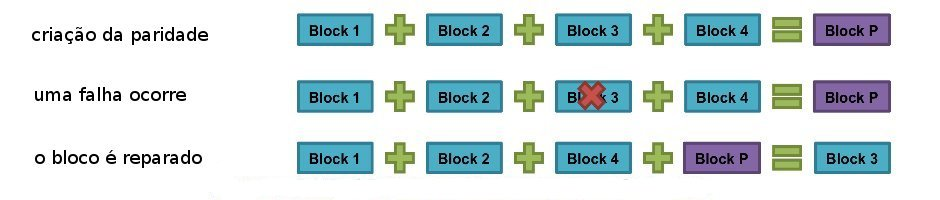
\includegraphics[scale=0.35]{raid5.jpg}
      \caption{RAID 5: 1 bloco de paridade e \emph{stripe} = 4 blocos \cite{MR-2036:2010}}
      \label{fig5:raid5}
    \end{figure}
 \end{frame}


  \begin{frame}{Motivação}
     \begin{itemize}
        \item Códigos Reed-Solomon (RS) são códigos de bloco, lineares e cíclicos (sobre anéis comutativos sob algumas condições).
        \item Parametrizáveis $===>$ capacidade de correção de erros pode ser alterada facilmente.
        \item RS são códigos MDS $===>$ as palavras-código apresentam máxima distância de Hamming entre si, permitida pelo número de dígitos de verificação de paridade do código.
        \item Segundo os autores em \cite{Almeida:2007,Sloane:1977}, códigos RS são úteis para correção de erros em rajada.
\begin{definition} {\bf Burst Errors} \index{Burst Errors} Uma sequência de erros em rajada ou \emph{burst errors} de tamanho $b$ é da forma:
    \begin{align*}
     (0, 0, \ldots, 0, 1, \ldots , 1, 0, \ldots, 0, 0)
    \end{align*}
onde o primeiro bit $1$ está na $i$-posição e o último bit $1$ está na $(i+b-1)$-posição e entre esses primeiro e último bits existe uma sequência de $b$ bits quaisquer.
\end{definition}
     \end{itemize}
  \end{frame}

% http://pic.dhe.ibm.com/infocenter/powersys/v3r1m5/index.jsp?topic=/arebk/raidsix.htm
  \begin{frame}{Motivação}
   \begin{figure}[h]
     \centering
     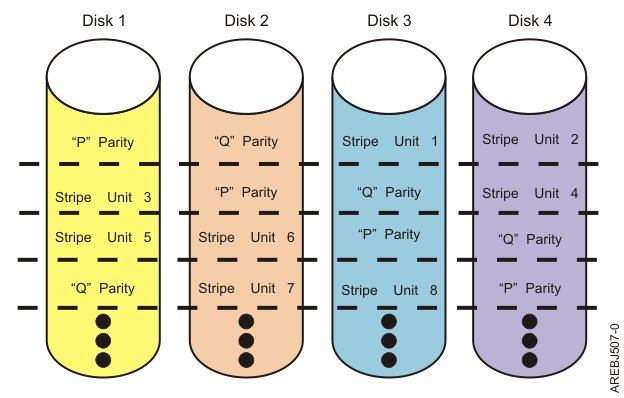
\includegraphics[scale=.4]{raid6.jpg}
     \caption{RAID 6 clássico "fatia" dados e paridade, através dos discos, como num arranjo. A paridade P e Q são geradas pela operação \emph{bitwise} XOR e pelo algoritmo Reed-Solomon.\cite{IBMR6:2012}}
     \label{fig6:raid6}
   \end{figure}
  \end{frame}

  \begin{frame}{Objetivos deste trabalho}

  \begin{itemize}
     \item avaliação de desempenho, ganhos, e custos de diferentes
  estratégias de códigos corretores de erro;
     \item implementação de otimizações ou extensões para o código fonte que
  atualmente implementa Reed-Solomon, tentando melhorar,
  principalmente, a parte de distribuição de blocos;
     \item implementação de novos algoritmos (Tornado e Turbo \emph{codes}) e
  extensão da interface atual para aceitá-los;
     \item integração do código fonte atual com o HDFS.
     \end{itemize}
  \end{frame}
